% Typestate Programming

\begin{frame}[fragile,t]{Typestate Programming 1}
    Den State mit dem Typ darstellen.

    \pause Beispiel:
    \begin{figure}
        \centering
        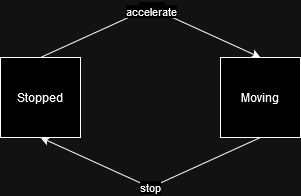
\includegraphics{images/typestate.drawio}
        \caption{Typestate Visualisierung}
        \label{fig:typestate-programming-1}
    \end{figure}
\end{frame}

\begin{frame}[fragile,t]{Typestate Programming 2}
    State "Stopped" initialisieren:
    \begin{lstlisting}[language=Rust,escapechar=@,label={lst:typestate-programming-2-1}]
let car_state: Stopped = Stopped::new();
println!("Starting at {} m", car_state.get_distance());
\end{lstlisting}
    \codeoutput{code/04-typestate1.txt}

    \pause zu State "Moving" übergehen
    \begin{lstlisting}[language=Rust,escapechar=@,label={lst:typestate-programming-2-2}]
let new_car_state: Moving = car_state.accelerate(
    5, // acceleration in m/s^2
    2 // how long to accelerate in seconds
);
println!("Accelerated to {} m/s", new_car_state.get_velocity());
\end{lstlisting}
    \codeoutput{code/04-typestate2.txt}
\end{frame}

\begin{frame}[fragile,t]{Typestate Programming 3}
    zurück zum State "Stopped"
    \begin{lstlisting}[language=Rust,escapechar=@,label={lst:typestate-programming-3-1}]
let final_car_state: Stopped = new_car_state.stop_after(
    10 // after how many seconds to stop moving
);

println!("Reached destination at {} m", final_car_state.get_distance());
    \end{lstlisting}
    \codeoutput{code/04-typestate3.txt}

\end{frame}
